\documentclass[11pt,a4paper]{article}

% ------------------------------------------------------------
% Packages
% ------------------------------------------------------------
\usepackage[utf8]{inputenc}
\usepackage[T1]{fontenc}
\usepackage[spanish,es-nodecimaldot]{babel}
\usepackage{lmodern}
\usepackage{geometry}
\usepackage{fancyhdr}
\usepackage{graphicx}
\usepackage[table]{xcolor}
\usepackage{booktabs}
\usepackage{longtable}
\usepackage{array}
\usepackage{tabularx}
\usepackage{enumitem}
\usepackage{hyperref}
\usepackage{parskip}
\usepackage{microtype}
\usepackage{tikz}
\usepackage{float}
\usepackage{titlesec}
\usepackage{caption}
\usepackage{listings}

\usetikzlibrary{arrows.meta,positioning,fit,calc,shapes.geometric,backgrounds,babel}

\geometry{margin=2.1cm, top=2.85cm, bottom=2.4cm, headheight=34pt}

\definecolor{livetixblue}{HTML}{173B57}
\definecolor{livetixaccent}{HTML}{C45C26}
\definecolor{livetixlight}{HTML}{EEF4F8}
\definecolor{livetixgray}{HTML}{5B6570}
\definecolor{livetixline}{HTML}{C5D0D8}
\definecolor{livetixok}{HTML}{2D6A4F}

\lstdefinestyle{livetixsql}{
    language=SQL,
    basicstyle=\ttfamily\footnotesize,
    keywordstyle=\bfseries\color{livetixblue},
    backgroundcolor=\color{livetixlight},
    frame=tb,
    rulecolor=\color{livetixline},
    framesep=6pt,
    breaklines=true,
    columns=fullflexible,
    keepspaces=true,
    showstringspaces=false,
    aboveskip=0.55em,
    belowskip=0.7em,
    morekeywords={interval}
}

\hypersetup{
    colorlinks=true,
    linkcolor=livetixblue,
    urlcolor=livetixblue,
    pdftitle={LiveTix --- Propuesta de arquitectura},
    pdfauthor={Rolando Palermo Rodríguez Cruz}
}

\titleformat{\section}
  {\Large\bfseries\color{livetixblue}}
  {\thesection.}{0.7em}{}
  [\color{livetixblue}\titlerule]
\titleformat{\subsection}
  {\large\bfseries\color{livetixblue}}
  {\thesubsection.}{0.6em}{}
\titleformat{\subsubsection}
  {\normalsize\bfseries\color{livetixblue}}
  {\thesubsubsection.}{0.5em}{}

\captionsetup{font=small, labelfont={bf,color=livetixblue}, skip=6pt}

\setlist[itemize]{leftmargin=*, itemsep=2pt, topsep=3pt}
\setlist[enumerate]{leftmargin=*, itemsep=2pt, topsep=3pt}

\newcommand{\sectionintro}[1]{\vspace{-0.15em}\textit{\textcolor{livetixgray}{#1}}\par\vspace{0.45em}}
\newcommand{\decision}[2]{\textbf{#1.} #2}

% Logo vectorial (ticket + wordmark). Si existe livetix-logo.png, se usa esa imagen.
\newcommand{\LiveTixLogoTikZ}{%
\begin{tikzpicture}[x=1mm, y=1mm, baseline=-1.1mm]
  \fill[livetixblue, rounded corners=1.4]
    (0,0) -- (28.6,0) -- (28.6,8.6) -- (0,8.6) -- cycle;
  \fill[white] (0,4.3) circle (1.35);
  \fill[white] (28.6,4.3) circle (1.35);
  \foreach \y in {1.3,2.6,3.9,5.2,6.5,7.8}
    \fill[white] (5.4,\y) circle (0.28);
  \node[white, font=\bfseries\sffamily, anchor=west, inner sep=0]
    at (7.0,4.35) {\fontsize{6.4}{7.4}\selectfont LiveTix};
\end{tikzpicture}%
}
\newcommand{\LiveTixLogo}[1][0.78cm]{%
  \IfFileExists{livetix-logo.png}{%
    \includegraphics[height=#1]{livetix-logo.png}%
  }{%
    \raisebox{-0.12cm}{\resizebox{!}{#1}{\LiveTixLogoTikZ}}%
  }%
}

\tikzset{
  lt/box/.style={
    draw=livetixblue, fill=livetixlight, rounded corners=2pt,
    align=center, inner sep=3.4pt, font=\sffamily\scriptsize, minimum height=7.2mm
  },
  lt/dark/.style={
    draw=livetixblue, fill=livetixblue, text=white, rounded corners=2pt,
    align=center, inner sep=3.4pt, font=\sffamily\scriptsize\bfseries, minimum height=7.2mm
  },
  lt/accent/.style={
    draw=livetixaccent, fill=livetixaccent, text=white, rounded corners=2pt,
    align=center, inner sep=3.4pt, font=\sffamily\scriptsize\bfseries, minimum height=7.2mm
  },
  lt/region/.style={
    draw=livetixblue, fill=white, rounded corners=3pt, inner sep=5pt,
    font=\sffamily\scriptsize
  },
  lt/arr/.style={-{Stealth[length=4.2pt]}, livetixblue, thick},
  lt/arrd/.style={-{Stealth[length=4.2pt]}, livetixgray, thick}
}

% ------------------------------------------------------------
% Header / Footer
% ------------------------------------------------------------
\pagestyle{fancy}
\fancyhf{}
\fancyhead[L]{%
  \parbox[c][0.78cm][c]{0.78\textwidth}{%
    \raggedright\sffamily\footnotesize\bfseries\color{livetixblue}%
    LiveTix --- Plataforma global de venta de boletos para eventos en vivo%
  }%
}
\fancyhead[R]{\LiveTixLogo[0.78cm]}
\fancyfoot[L]{\sffamily\scriptsize\textcolor{livetixgray}{Propuesta de arquitectura}}
\fancyfoot[R]{\sffamily\scriptsize\textcolor{livetixgray}{\thepage}}
\renewcommand{\headrulewidth}{0.6pt}
\renewcommand{\footrulewidth}{0.3pt}
\renewcommand{\headrule}{\hbox to\headwidth{\color{livetixblue}\leaders\hrule height \headrulewidth\hfill}}
\renewcommand{\footrule}{\hbox to\headwidth{\color{livetixline}\leaders\hrule height \footrulewidth\hfill}}

\begin{document}

% ------------------------------------------------------------
% Title
% ------------------------------------------------------------
\pagenumbering{Alph}
\begin{titlepage}
    \thispagestyle{empty}
    \noindent
    \begin{tikzpicture}
      \fill[livetixblue] (0,0) rectangle (\textwidth, 0.18cm);
    \end{tikzpicture}

    \vspace*{1.8cm}
    \begin{flushright}
        \LiveTixLogo[1.15cm]
    \end{flushright}

    \vspace{1.6cm}
    {\Huge\bfseries\sffamily\textcolor{livetixblue}{Propuesta de arquitectura}}\\[0.45cm]
    {\Large\sffamily Plataforma global de venta de boletos para eventos en vivo}\\[1.0cm]
    {\color{livetixaccent}\rule{4.2cm}{2.4pt}}\\[0.7cm]
    {\large\sffamily System Design Challenge}

    \vfill
    \begin{tabular}{@{}ll}
        \textbf{Autor} & Rolando Palermo Rodríguez Cruz \\
        \textbf{Fecha} & 06 de septiembre de 2026 \\
        \textbf{Versión} & 1.0 \\
        \textbf{Clasificación} & Propuesta técnica \\
    \end{tabular}

    \vspace{1.4cm}
    \noindent
    \begin{tikzpicture}
      \fill[livetixblue] (0,0) rectangle (\textwidth, 0.18cm);
    \end{tikzpicture}
\end{titlepage}

\clearpage
\pagenumbering{arabic}
\setcounter{page}{1}

% ------------------------------------------------------------
% Change control
% ------------------------------------------------------------
\section*{Control de cambios}
\addcontentsline{toc}{section}{Control de cambios}

\renewcommand{\arraystretch}{1.4}
\begin{tabularx}{\textwidth}{>{\raggedright\arraybackslash}p{4.4cm}
                             >{\centering\arraybackslash}p{2.6cm}
                             >{\raggedright\arraybackslash}X}
\rowcolor{livetixblue}
\textcolor{white}{\textbf{Autor}} &
\textcolor{white}{\textbf{Fecha}} &
\textcolor{white}{\textbf{Descripción}} \\
Rolando Palermo Rodríguez Cruz & 06/09/2026 &
Versión inicial de la propuesta: arquitectura global, decisiones técnicas e infraestructura como código / CI/CD. \\
\end{tabularx}
\renewcommand{\arraystretch}{1.0}

\vspace{1.1cm}
\tableofcontents
\clearpage

% ============================================================
\section{Diagrama de arquitectura}
% ============================================================

\sectionintro{La arquitectura está pensada para operar en cuatro países, absorber picos de 10 a 20 veces el tráfico habitual y proteger dos invariantes: no vender dos veces el mismo asiento y no capturar un pago sin boleto.}

\subsection{Contexto y alcance}

LiveTix opera en México, Estados Unidos, España y Japón. La propuesta usa tres regiones de AWS:

\begin{center}
\renewcommand{\arraystretch}{1.25}
\begin{tabular}{lll}
\toprule
\textbf{Región AWS} & \textbf{Mercados} \\
\midrule
\texttt{us-east-1} & México y Estados Unidos \\
\texttt{eu-west-1} & España \\
\texttt{ap-northeast-1} & Japón \\
\bottomrule
\end{tabular}
\end{center}

\begin{itemize}
    \item La capa global \textit{Route~53} +  \textit{CloudFront} +  \textit{WAF} es única.
    \item Los servicios de aplicación y los datos transaccionales se despliegan por región.
    \item Cada evento tiene una \textit{home region}.
    \item Las lecturas no críticas (catálogo de eventos, información del evento, imágenes/banners, recomendaciones, etc.) pueden resolverse cerca del usuario.
    \item La reserva y la venta de asientos siempre se escriben en la región propietaria del evento.
\end{itemize}

\subsection{Arquitectura lógica}

\begin{figure}[H]
\centering
\resizebox{\textwidth}{!}{%
\begin{tikzpicture}[font=\sffamily\scriptsize, x=1cm, y=1cm]
  % --- Usuarios ---
  \draw[livetixblue, fill=livetixlight, rounded corners=3pt]
    (0,12.40) rectangle (15.2,14.30);
  \node[font=\sffamily\bfseries\color{livetixblue}] at (7.6,14.05) {Usuarios};
  \node[lt/box, minimum width=4.2cm, fill=white] (amer) at (2.6,13.00) {USA/MX};
  \node[lt/box, minimum width=4.2cm, fill=white] (emea) at (7.6,13.00) {ES};
  \node[lt/box, minimum width=4.2cm, fill=white] (apac) at (12.6,13.00) {JPN};

  % --- Borde global (columna vertical) ---
  \draw[livetixblue, fill=white, rounded corners=3pt]
    (4.15,7.50) rectangle (11.05,12.15);
  \node[font=\sffamily\bfseries\color{livetixblue}] at (7.6,11.88) {Borde global};
  \node[lt/box, minimum width=6.4cm] (r53) at (7.6,10.90) {Route 53\\DNS global};
  \node[lt/box, minimum width=6.4cm] (cf) at (7.6,9.70) {CloudFront\\CDN};
  \node[lt/box, minimum width=6.4cm] (waf) at (7.6,8.50) {AWS WAF\\per\'imetro};

  % --- Waiting Room ---
  \draw[livetixblue, fill=white, rounded corners=3pt]
    (0,5.15) rectangle (15.2,7.30);
  \node[font=\sffamily\bfseries\color{livetixblue}] at (7.6,7.03)
    {Waiting Room / Admission Service};
  \node[lt/accent, minimum width=6.8cm] (wr) at (4.0,6.05) {Admission Service\\Lambda@Edge};
  \node[lt/box, minimum width=6.8cm] (ddb) at (11.2,6.05) {DynamoDB\\Queue State};

  \node[lt/region, minimum width=4.6cm] (us) at (2.6,3.15) {%
    \begin{tabular}{@{}c@{}}
      \textbf{\textcolor{livetixblue}{us-east-1}}\\[1pt]
      {\scriptsize home MX / US}\\[3pt]
      Catalog · Checkout\\
      Inventory · Ticket\\
      Reconciliation Job\\[2pt]
      ECS / Fargate Multi-AZ\\[2pt]
      Aurora PostgreSQL (SoT)\\
      Redis · SQS · S3
    \end{tabular}
  };
  \node[lt/region, minimum width=4.6cm] (eu) at (7.6,3.15) {%
    \begin{tabular}{@{}c@{}}
      \textbf{\textcolor{livetixblue}{eu-west-1}}\\[1pt]
      {\scriptsize home ES}\\[3pt]
      Catalog · Checkout\\
      Inventory · Ticket\\
      Reconciliation Job\\[2pt]
      ECS / Fargate Multi-AZ\\[2pt]
      Aurora PostgreSQL (SoT)\\
      Redis · SQS · S3
    \end{tabular}
  };
  \node[lt/region, minimum width=4.6cm] (ap) at (12.6,3.15) {%
    \begin{tabular}{@{}c@{}}
      \textbf{\textcolor{livetixblue}{ap-northeast-1}}\\[1pt]
      {\scriptsize home JP}\\[3pt]
      Catalog · Checkout\\
      Inventory · Ticket\\
      Reconciliation Job\\[2pt]
      ECS / Fargate Multi-AZ\\[2pt]
      Aurora PostgreSQL (SoT)\\
      Redis · SQS · S3
    \end{tabular}
  };

  \node[lt/box, minimum width=15.0cm] (ops) at (7.6,0.75) {%
    Secrets Manager / KMS \quad·\quad CloudWatch \quad·\quad IAM \quad·\quad ECR
  };

  \draw[lt/arr] (amer.south) -- (r53.north west);
  \draw[lt/arr] (emea.south) -- (r53.north);
  \draw[lt/arr] (apac.south) -- (r53.north east);
  \draw[lt/arr] (r53.south) -- (cf.north);
  \draw[lt/arr] (cf.south) -- (waf.north);
  \draw[lt/arr] (waf.south) -- (wr.north);
  \draw[lt/arr] (wr.south) -- (us.north);
  \draw[lt/arr] (wr.south) -- (eu.north);
  \draw[lt/arr] (wr.south) -- (ap.north);
\end{tikzpicture}%
}
\caption{Arquitectura global de LiveTix: usuarios entran por Route~53 hacia CloudFront y WAF; Waiting Room en Lambda@Edge con DynamoDB; tres regiones con fuente de verdad local y job de reconciliación.}
\end{figure}

\subsection{Flujos críticos}

\subsubsection{Flash crowd y control de admisión}

Cuando se liberan boletos, el sistema no espera a que ECS reaccione. En su lugar:
\begin{itemize}
\item Route~53 resuelve el DNS; CloudFront y WAF absorben y filtran.
\item La sala de espera (Admission Service en Lambda@Edge) dosifica el ingreso al checkout; DynamoDB guarda el estado de la cola.
\item La capacidad de Fargate se preescala antes del evento.
\end{itemize}

\clearpage
\begin{figure}[p]
\centering
\includegraphics[width=\textwidth,height=0.84\textheight,keepaspectratio]{checkout-api-admission-flow.png}
\caption{Flujo de admisión al checkout. CloudFront y WAF filtran; Admission Service y DynamoDB dosifican el ingreso antes de Fargate.}
\end{figure}
\clearpage

\subsubsection{Concurrencia de inventario}

La reserva es una actualización condicional en Aurora. El asiento pasa de \texttt{AVAILABLE} a \texttt{HELD} y después a \texttt{SOLD}, o regresa a \texttt{AVAILABLE} si el hold expira.

\begin{itemize}
\item El \texttt{hold\_id} es el token de propiedad temporal.
\item El worker de expiración es idempotente: no puede liberar un hold nuevo que ya sustituyó al anterior.
\end{itemize}

\clearpage
\begin{figure}[p]
\centering
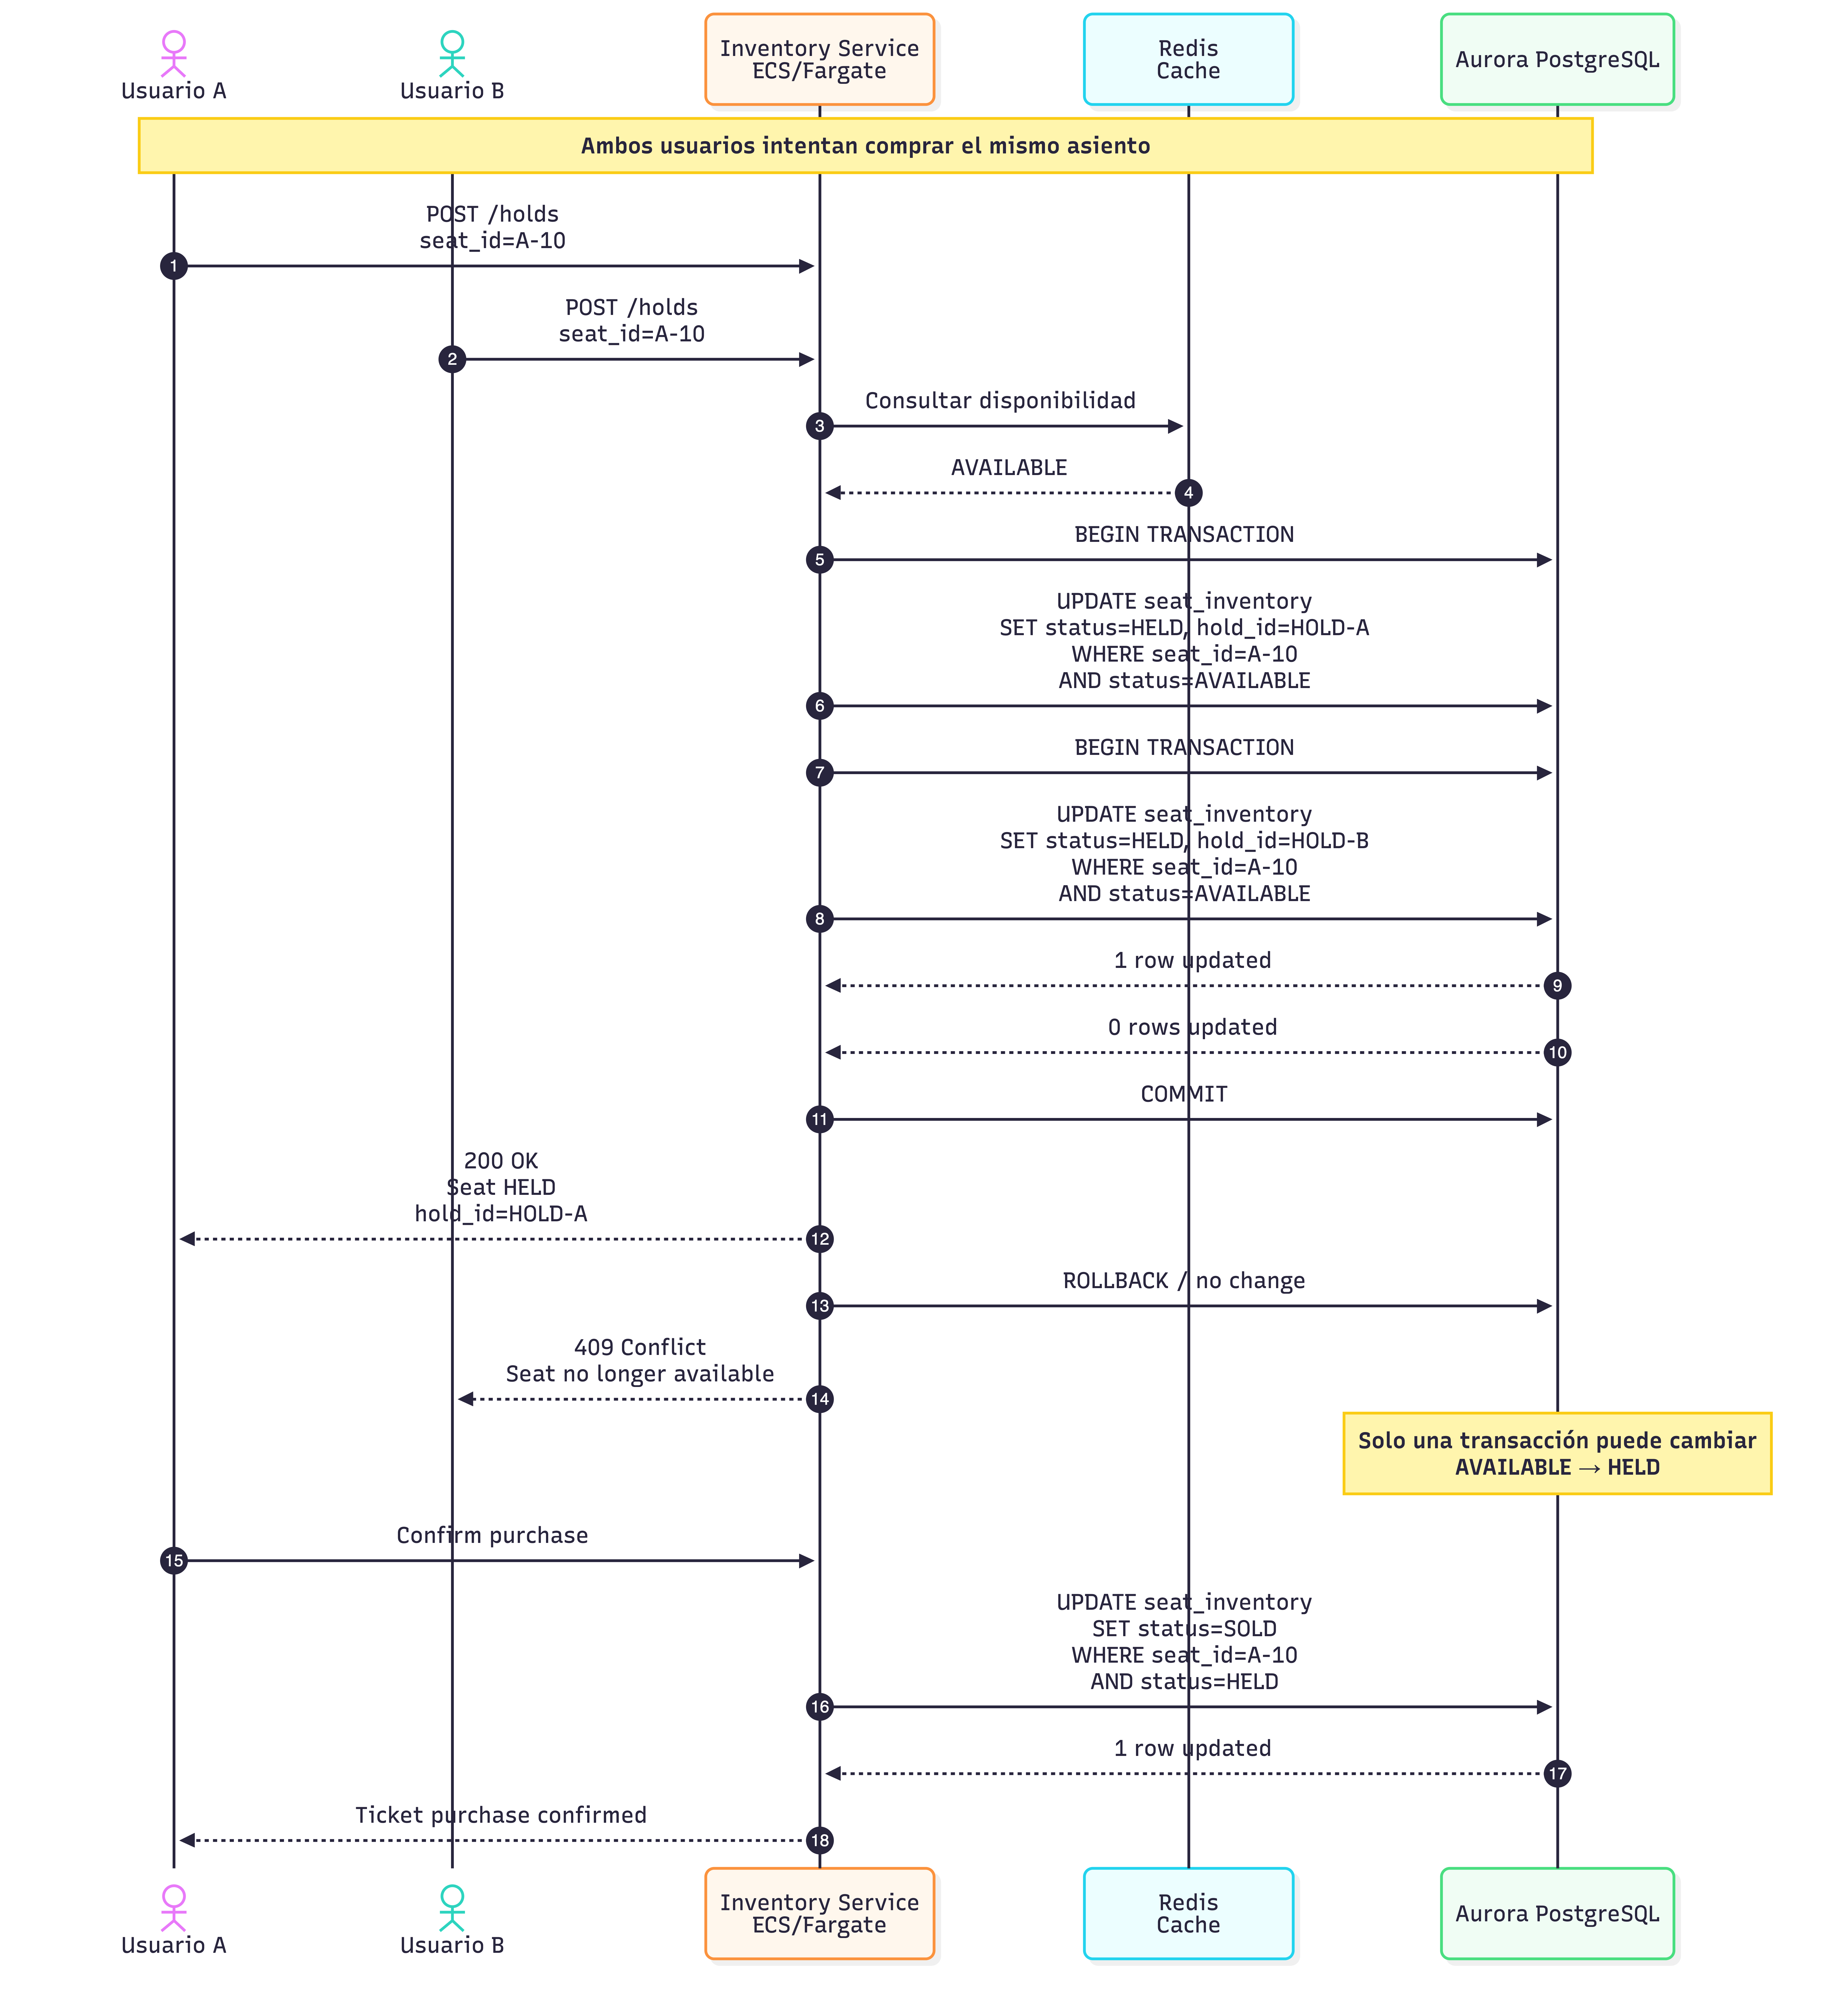
\includegraphics[width=\textwidth,height=0.84\textheight,keepaspectratio]{concurrencia_inventario_sequence_diagram.png}
\caption{Concurrencia de inventario. Dos compradores intentan el mismo asiento; Aurora confirma un solo hold.}
\end{figure}
\clearpage

\subsubsection{Pago, boleto y conciliación}

El hold del asiento queda en el flujo de inventario. La autorización, la emisión del boleto, la captura y la conciliación se detallan en la sección de consistencia de pago (Figura~\ref{fig:pago-boleto}).

% ============================================================
\section{Decisiones importantes}
% ============================================================

\sectionintro{Las decisiones privilegian consistencia, absorción de picos y una operación que un equipo de cinco ingenieros pueda sostener.}

\subsection{Inventario como fuente de verdad}

\decision{Aurora PostgreSQL es la autoridad del asiento}{El inventario numerado exige exclusión mutua. Una actualización condicional (\texttt{status = AVAILABLE}) más una restricción de unicidad evitan la doble venta.}

\textbf{Reserva atómica.} Solo actualiza el asiento si sigue \texttt{AVAILABLE}:

\begin{lstlisting}[style=livetixsql]
UPDATE seat_inventory
SET status = 'HELD',
    hold_id = :hold_id,
    hold_expires_at = now() + interval '5 minutes'
WHERE event_id = :event_id
  AND seat_id = :seat_id
  AND status = 'AVAILABLE';
\end{lstlisting}

\textbf{Liberación de asiento.} El worker solo libera el hold que le corresponde y que ya venció:

\begin{lstlisting}[style=livetixsql]
UPDATE seat_inventory
SET status = 'AVAILABLE',
    hold_id = NULL,
    hold_expires_at = NULL
WHERE event_id = :event_id
  AND seat_id = :seat_id
  AND status = 'HELD'
  AND hold_id = :hold_id
  AND hold_expires_at <= NOW();
\end{lstlisting}

Si el \texttt{UPDATE} de reserva afecta 0 filas, otro comprador ya tomó el asiento. La condición \texttt{hold\_id = :hold\_id} en la liberación hace que un worker retrasado no deshaga un hold posterior.

\subsection{Picos de tráfico}

El autoescalado reactivo llega tarde cuando la demanda crece en segundos. La defensa es en capas:

\begin{itemize}
    \item Preescalado de Fargate antes de eventos anunciados.
    \item CloudFront para lo estático y cacheable.
    \item WAF en el perímetro.
    \item Waiting Room para dosificar el checkout.
    \item SQS para trabajo asíncrono que no debe competir con la reserva.
\end{itemize}

El objetivo no es que todos lleguen al mismo tiempo al asiento, sino que quienes pasan el cupo encuentren un sistema estable.

\subsection{Consistencia de pago}

La pasarela es dueña del instrumento; LiveTix es dueño de la orden, el asiento y el boleto. La integración usa claves de idempotencia. Autorizar y capturar van separados a propósito: no se cobra en firme si todavía no hay boleto. El flujo, a partir de una orden ya en hold, se muestra en la Figura~\ref{fig:pago-boleto}.

\begin{figure}[H]
\centering
\includegraphics[width=\textwidth,height=0.72\textheight,keepaspectratio]{checkout-api-admission-flow-060456.png}
\caption{Pago, boleto y conciliación. La captura ocurre después de emitir el boleto; si la emisión falla de forma permanente se hace \textit{void} y un reconciliador cierra huecos entre sistemas.}
\label{fig:pago-boleto}
\end{figure}

\subsection{Transactional outbox e idempotencia}

El evento de emisión se persiste en la misma transacción que confirma asiento y orden. Un publisher aparte lo coloca en SQS. Los consumidores asumen entrega \textit{at-least-once}: la generación del boleto y la captura deben ser idempotentes.

\subsection{Multi-región y resiliencia}

Cada región corre en varias Availability Zones. La escritura crítica no cruza de región en el camino feliz. Ante una caída regional completa se recupera en una región secundaria; RPO y RTO se confirman con pruebas de failover, no solo con el diseño.

\subsection{Observabilidad}

Alarmas prioritarias:

\begin{itemize}
    \item Tasa de éxito de checkout.
    \item Conflictos de reserva de inventario.
    \item Fallos de autorización y de captura.
    \item Latencia y errores de emisión de boletos.
    \item Profundidad y antigüedad de SQS.
    \item Órdenes sin boleto.
    \item Pagos sin boleto correspondiente.
    \item Errores por región y por Availability Zone.
\end{itemize}

La métrica de negocio que no puede quedar en verde con mentiras es \texttt{payment\_ticket\_inconsistency = 0}.

\subsection{Tradeoffs principales}

\begin{longtable}{p{3.8cm} p{5.2cm} p{5.2cm}}
\toprule
\textbf{Decisión} & \textbf{Beneficio} & \textbf{Costo} \\
\midrule
\endfirsthead
\toprule
\textbf{Decisión} & \textbf{Beneficio} & \textbf{Costo} \\
\midrule
\endhead
\textit{Home region} por evento & Consistencia fuerte del inventario & Una compra puede cruzar región \\
Aurora como fuente de verdad & Evita double-selling & Más costo que un cache puro \\
Waiting Room & Protege el checkout en picos & El usuario espera \\
SQS + outbox & Absorbe carga y sobrevive a fallos parciales & Más piezas que operar \\
Fargate & Menos servidores que administrar & Menos control fino que EC2 \\
Multi-AZ + DR regional & Resiliencia real & Costo y ejercicios de failover \\
Sin K8s ni service mesh & Operable por un equipo pequeño & Menos portabilidad multi-cloud \\
\bottomrule
\end{longtable}

% ============================================================
\section{Infraestructura como código \& CI/CD}
% ============================================================

\sectionintro{Terraform y el pipeline tienen que permitir levantar ambientes de forma repetible, aislar las regiones y hacer despliegues sin que terminemos manteniendo una plataforma paralela que se vuelva demasiado pesada para un equipo de cinco personas. El state de Terraform se mantiene en un bucket S3 dedicado, con versionado, cifrado y acceso controlado por IAM, para evitar perderlo o que alguien lo modifique directamente.}

\subsection{Estructura de Terraform}

\begin{verbatim}
infrastructure/
|
+-- modules/
|   +-- networking/
|   +-- ecs/
|   +-- aurora/
|   +-- redis/
|   +-- sqs/
|   +-- dynamodb/
|   +-- waf/
|   +-- waiting-room/
|   +-- secrets/
|   +-- observability/
|
+-- environments/
|   +-- dev/
|   +-- staging/
|   +-- production/
|       +-- us-east-1/
|       +-- eu-west-1/
|       +-- ap-northeast-1/
|
+-- global/
    +-- route53/
    +-- cloudfront/
    +-- iam/
\end{verbatim}

\begin{itemize}
    \item Los módulos expresan el patrón reutilizable (servicio ECS, cluster Aurora, cola, tabla DynamoDB, WAF, Waiting Room, secretos, observabilidad).
    \item CloudFront vive solo en \texttt{global/}. El Waiting Room es Lambda@Edge asociado a esa distribución; WAF se adjunta al mismo borde.
    \item Los environments solo pasan capacidad, red y flags, e instancian \texttt{modules/secrets} por ambiente.
    \item Producción se parte por región para limitar el blast radius.
    \item Los recursos globales (Route~53, CloudFront y IAM) viven fuera de los stacks regionales.
\end{itemize}

\subsection{Versionado y cambios}

Versiones de módulos y providers van fijadas. Todo cambio entra por pull request, con \texttt{terraform plan} en CI y apply solo después de revisión.

\subsection{Secretos}

Nada de secretos en git ni en \texttt{tfvars} versionados. Secrets Manager y KMS, con IAM de mínimo privilegio y roles de tarea en lugar de access keys estáticas.

\subsection{Pipeline CI/CD}

\begin{figure}[H]
\centering
\resizebox{\textwidth}{!}{%
\begin{tikzpicture}[font=\sffamily\scriptsize, node distance=6mm and 4.2mm]
  \node[lt/box, minimum width=2.6cm, minimum height=1.65cm, align=center] (pr)
    {PR\\compilación, tests\\y quality gates};
  \node[lt/box, minimum width=2.6cm, minimum height=1.65cm, align=center, right=of pr] (img)
    {Imagen Docker\\build};
  \node[lt/box, minimum width=2.6cm, minimum height=1.65cm, align=center, right=of img] (scan)
    {Scan\\dependencias\\e imagen};
  \node[lt/box, minimum width=2.6cm, minimum height=1.65cm, align=center, right=of scan] (ecr)
    {ECR\\publicar imagen};
  \node[lt/box, minimum width=2.6cm, minimum height=1.65cm, align=center, right=of ecr] (dev)
    {Dev\\deploy automático};

  \node[lt/box, minimum width=2.6cm, minimum height=1.65cm, align=center, below=14mm of pr] (stg)
    {Staging\\integración\\y smoke};
  \node[lt/accent, minimum width=2.6cm, minimum height=1.65cm, align=center, right=of stg] (appr)
    {Aprobación\\producción};
  \node[lt/dark, minimum width=2.6cm, minimum height=1.65cm, align=center, right=of appr] (prod)
    {Prod\\canary o\\blue/green};
  \node[lt/box, minimum width=2.6cm, minimum height=1.65cm, align=center, right=of prod] (obs)
    {Métricas\\verificar alarmas};
  \node[lt/box, minimum width=2.6cm, minimum height=1.65cm, align=center, right=of obs] (rb)
    {Rollback\\si hay alarma};

  \draw[lt/arr] (pr) -- (img);
  \draw[lt/arr] (img) -- (scan);
  \draw[lt/arr] (scan) -- (ecr);
  \draw[lt/arr] (ecr) -- (dev);
  \draw[lt/arr] (dev.south) -- ++(0,-0.42) -| (stg.north);
  \draw[lt/arr] (stg) -- (appr);
  \draw[lt/arr] (appr) -- (prod);
  \draw[lt/arr] (prod) -- (obs);
  \draw[lt/arr] (obs) -- (rb);
\end{tikzpicture}%
}
\caption{Pipeline: verificación automática hasta staging; producción con aprobación, canary y rollback por alarmas.}
\end{figure}

Infraestructura sigue un pipeline paralelo: \texttt{fmt}, \texttt{validate}, \texttt{plan} en el PR y \texttt{apply} controlado por ambiente. Las migraciones de base de datos deben ser compatibles con el código anterior para no romper un canary a medias.

% ============================================================
\section*{Conclusión}
\addcontentsline{toc}{section}{Conclusión}

\begin{enumerate}
    \item La propuesta no maximiza sofisticación. Busca tres garantías: el checkout no colapsa en un flash crowd, un asiento se vende una sola vez y una captura de pago tiene boleto.
    \item Outbox, consumidores idempotentes y reconciliación cubren los huecos entre LiveTix y la pasarela.
    \item Terraform, ambientes aislados y un pipeline con canary permiten operar esto con un equipo pequeño.
\end{enumerate}
\end{document}
